\chapter{生态系统动态}\label{ch:b1:ecosystem-dynamics}

北太平洋某冰川已退缩了两个世纪，从其冰舌
沿峡湾往回走，便是一段穿越时间的旅程。
去年刚露出的岩石裸露无物；再往前一千米，
岩面上长着苔藓和\omterm{def:b1:plant-water-minerals:nodules}{固氮}的垫状植被；再往前是
桤木丛，然后是云杉，再后是两百年树龄的
云杉与铁杉林，其下覆盖着一米厚的土壤。这里没有任何东西是静止的：
每一次\omterm{def:b1:ecosystem-dynamics:disturbance}{干扰}之后，\omterm{def:b1:ecosystem-organization:ecosystem}{生态系统}都会变化，其路径
部分可以预测，而它们保留和循环养分的能力也随之改变。
本章讨论这些变化——
\omterm{def:b1:ecosystem-dynamics:succession}{演替}、\omterm{def:b1:ecosystem-dynamics:disturbance}{干扰}与恢复、养分的保持、
岛屿上\omterm{def:b1:ecosystem-organization:ecosystem}{群落}的组装——以及那些使其
从叙述变为数据的实验。

\section{演替}

\begin{definition}[生态演替]\label{def:b1:ecosystem-dynamics:succession}
\index{演替}\index{初生演替}\index{次生演替}\index{顶极群落}
\emph{演替}是指\omterm{def:b1:ecosystem-organization:ecosystem}{群落}在一次\omterm{def:b1:ecosystem-dynamics:disturbance}{干扰}之后随时间发生的定向变化，
一组物种依次取代另一组，直至一个相对稳定的\omterm{def:b1:ecosystem-organization:ecosystem}{群落}
即\emph{顶极\omterm{def:b1:ecosystem-organization:ecosystem}{群落}}，得以维持。\emph{初生
演替}始于缺乏土壤和\omterm{def:b1:organism-environment:organism}{生物体}的新基质，
如冰川留下的岩石、熔岩流、沙丘和新形成的岛屿。
\emph{次生演替}始于\omterm{def:b1:ecosystem-organization:ecosystem}{群落}已遭毁坏但土壤及种子库仍存的地方，
例如被弃耕的农田、
被烧毁或砍伐的森林、被淹没的草甸。最早到来的是\emph{先锋物种}，
它们是善于扩散、能耐受裸地的物种；
较晚到来的则是耐阴、需要土壤的竞争者。
\end{definition}

\begin{proposition}[替代的机制]\label{prop:b1:ecosystem-dynamics:mechanisms}
\index{促进}
\omterm{def:b1:ecosystem-dynamics:succession}{演替}的每一阶段都可以以三种方式促成下一阶段。
\emph{促进}：较早的物种使该地点适合后来者，
使后来者得以定居——营造土壤、固定氮素、投下荫蔽，
保持水分，然后被后者取代。\emph{抑制}：
先到的居民抵御一切来者，直到死亡或受损，
此后取代它们的，是届时恰好到达的物种。
\emph{耐受}：后来的物种同样在起点到达，生长缓慢，
并最终比先锋物种存活得更久，而先锋物种的存在
对它们既无帮助也无妨碍。大多数\omterm{def:b1:ecosystem-dynamics:succession}{演替}在不同
阶段同时呈现这三种方式；\omterm{def:b1:ecosystem-dynamics:succession}{初生演替}以促进为主，
因为首要任务是造出土壤。
\end{proposition}
\begin{proof}[证据]
在阿拉斯加的冰川湾，冰川已退缩了
自 1750 年以来约\qty{100}{km}，各地点的年龄可由地图与树轮得知，
并可按顺序依次考察各阶段：裸露冰碛土、
蓝细菌与苔藓形成的皮壳，以及\omterm{def:b1:plant-water-minerals:nodules}{固氮}的
\emph{Dryas} 构成的垫状\omterm{def:b1:ecosystem-organization:ecosystem}{群落}，桤木丛（\omterm{def:b1:plant-water-minerals:nodules}{固氮}，每年每公顷
新增\qty{50}{kg}氮），然后是锡特卡云杉，
两个世纪后出现云杉–铁杉林。土壤氮含量由几乎为零
升至桤木丛下的\qty{300}{kg/ha}，
云杉只能在桤木之后定居；\omterm{def:b1:water-small-molecules:ph}{pH} 由 8 降至 5 以下，
随\omterm{def:b1:ecosystem-dynamics:decomposition}{凋落物}积累。种在幼龄冰碛土上的云杉幼苗
只有施加氮肥才能生长，可见桤木是促进者。
\end{proof}

\begin{omfigure}
\begin{tikzpicture}[font=\footnotesize, >=Stealth, line cap=round]
  \draw[->, thick] (0,0) -- (12.2,0); \node[anchor=north] at (6.0,-0.45) {冰川退去以来的年数};
  \foreach \x/\l in {0/0, 2.4/20, 4.8/50, 7.2/100, 9.6/150, 12.0/200} { \draw (\x,0.08) -- (\x,-0.08) node[below] {\l}; }
  \fill[gray!30] (0,0.15) rectangle (1.4,0.55); \node[anchor=south] at (0.7,0.6) {裸露冰碛土};
  \fill[omExo!30] (1.0,0.15) rectangle (3.4,0.55); \node[anchor=south, align=center] at (2.4,0.6) {苔藓、\emph{Dryas}\\（固氮）};
  \fill[omProp!35] (3.0,0.15) rectangle (6.4,0.55); \node[anchor=south, align=center] at (4.9,0.6) {桤木丛 \\（\qty{50}{kg} N/ha/yr）};
  \fill[omDef!30] (5.8,0.15) rectangle (9.8,0.55); \node[anchor=south] at (8.0,0.6) {云杉林};
  \fill[omThm!30] (9.2,0.15) rectangle (12.0,0.55); \node[anchor=south] at (10.6,0.6) {云杉–铁杉};
  % soil nitrogen curve
  \begin{scope}[yshift=2.0cm]
    \draw[->, thick] (0,0) -- (0,2.6) node[above] {土壤 N（\unit{kg/ha}）};
    \foreach \y/\l in {0/0, 0.8/100, 1.6/200, 2.4/300} { \draw (-0.08,\y) -- (0.08,\y) node[left=4pt] {\l}; }
    \draw[very thick, omProp!80!black] plot[smooth] coordinates {(0,0.02) (1.4,0.1) (3.0,0.5) (4.8,1.6) (6.4,2.3) (8.0,2.4) (12.0,2.3)};
    \draw[very thick, omThm, dashed] plot[smooth] coordinates {(0,2.5) (2.4,2.3) (4.8,1.5) (7.2,0.9) (9.6,0.6) (12.0,0.5)};
    \node[omThm, anchor=west] at (12.1,0.5) {pH（8 至 4.5）};
    \node[omProp!80!black, anchor=west] at (12.1,2.3) {N};
  \end{scope}
\end{tikzpicture}

{\small 冰川湾的\omterm{def:b1:ecosystem-dynamics:succession}{初生演替}：各阶段按地点年龄排列，
土壤氮含量在\omterm{def:b1:plant-water-minerals:nodules}{固氮}的桤木丛下升高，
\omterm{def:b1:water-small-molecules:ph}{pH} 随\omterm{def:b1:ecosystem-dynamics:decomposition}{凋落物}积累而下降。云杉
在桤木营造出土壤之后才出现。}
\end{omfigure}

\begin{omfigure}
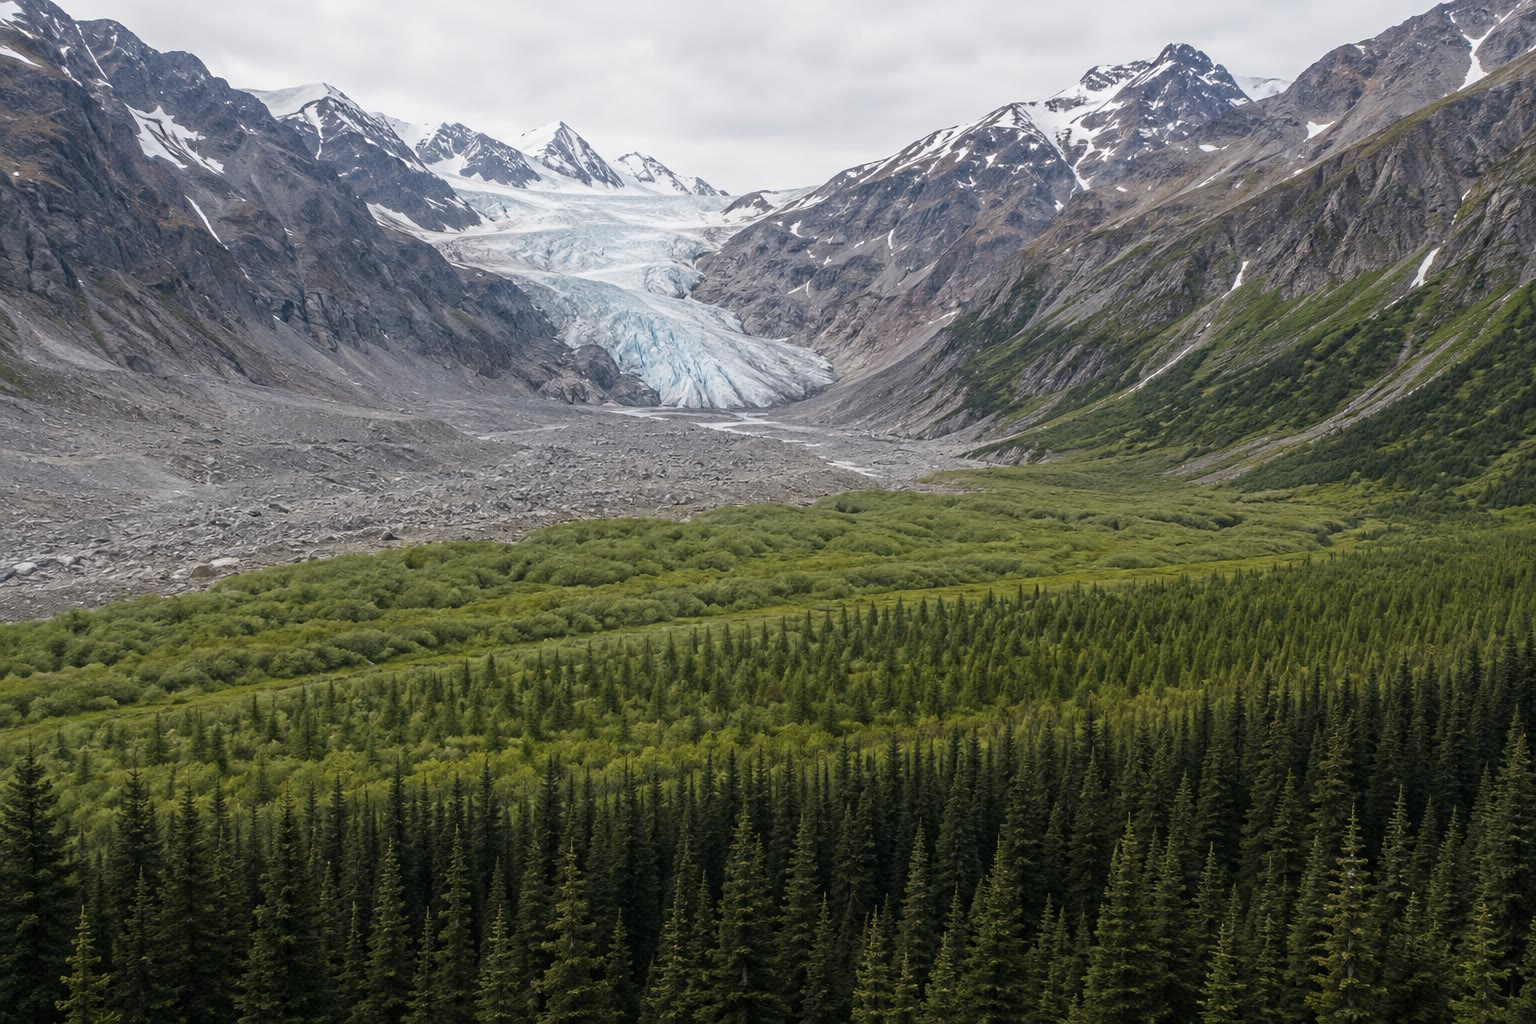
\includegraphics[width=0.62\linewidth]{images/book3/ai/b3-28-glacier-succession.jpg}

{\small 将一条退缩中的冰川谷视为一个时间序列：紧贴冰体的
裸露冰碛垄，随后是矮灌丛，再后是针叶林，
位于裸露时间最长的地面上。}
\end{omfigure}

\begin{example}[一块弃耕地]\label{ex:b1:ecosystem-dynamics:oldfield}
美国东部一块被弃耕的田地，第一年
即由种子库和风带来的一年生杂草（马唐、豚草）占据；
第三年，多年生草本和一枝黄花占优势；
第十年出现灌木和松树幼苗；第二十五年形成松林，
林下松树自己的幼苗无法生长，
而栎树和山核桃树的幼苗却可以；至第一百年，形成栎–山核桃林，
其幼苗能耐受林荫，因此得以自我更新。
每一阶段都被这样一些物种取代：它们的扩散能力
不及前一阶段，而竞争力更强；土壤从一开始就已存在，
整个\omterm{def:b1:ecosystem-dynamics:succession}{演替}序列所需时间约为人的一生，
而\omterm{def:b1:ecosystem-dynamics:succession}{初生演替}则需数千年。
\end{example}

\begin{omfigure}
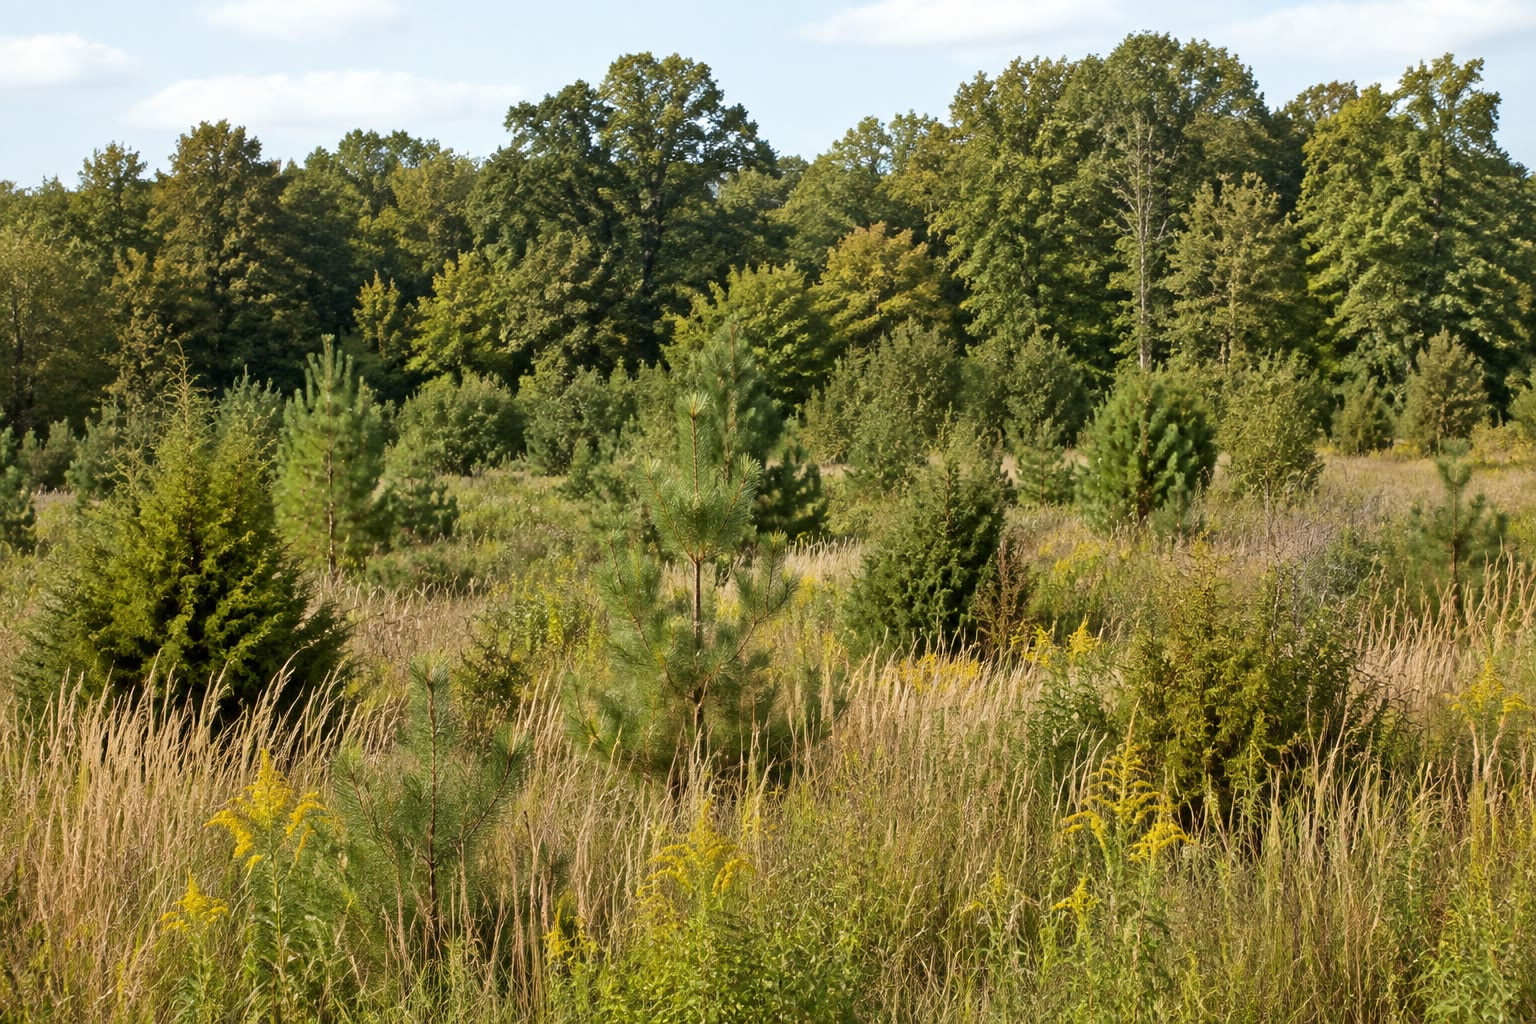
\includegraphics[width=0.6\linewidth]{images/book3/ai/b3-28-old-field.jpg}

{\small 废弃田地中的\omterm{def:b1:ecosystem-dynamics:succession}{次生演替}：前景为一枝黄花与禾草，
后方为幼龄松树与刺柏，
最远处为将取代它们的落叶林。}
\end{omfigure}

\begin{omfigure}
\begin{tikzpicture}
\begin{axis}[
  width=0.8\linewidth, height=6.2cm,
  axis x line=bottom, axis y line=left,
  xmin=0, xmax=160, ymin=0, ymax=1.15,
  xlabel={弃耕后年数}, ylabel={相对量},
  xlabel style={font=\small}, ylabel style={font=\small},
  tick label style={font=\small}, ytick={0,0.5,1},
  legend style={font=\scriptsize, at={(0.98,0.03)}, anchor=south east, draw=none, fill=none},
  legend cell align=left,
]
\addplot[omExo!80!black, very thick, domain=0:160, samples=80] {1/(1+exp(-(x-40)/12))};
\addlegendentry{生物量（占顶极群落的比例）}
\addplot[omDef, very thick, domain=0:160, samples=80] {0.3 + 0.8*x/60*exp(1-x/60)};
\addlegendentry{物种丰富度}
\addplot[omThm, very thick, domain=0:160, samples=80] {1.0*exp(-x/25)*(x<25) + (0.37 + 0.4*(1-exp(-(x-25)/30)))*(x>=25)};
\addlegendentry{净生产量 / 生物量}
\end{axis}
\end{tikzpicture}

{\small \omterm{def:b1:ecosystem-dynamics:succession}{次生演替}中的变化趋势（示意）。生物量
上升至平台期；\omterm{def:b1:ecosystem-organization:diversity}{物种丰富度}在中途达到峰值，此时先锋物种与后期物种
并存；随着\omterm{def:b1:ecosystem-organization:ecosystem}{群落}被木质\omterm{def:b1:body-plans-tissues:tissue}{组织}填充，净生产量与生物量之比下降，
这些木质\omterm{def:b1:body-plans-tissues:tissue}{组织}消耗呼吸作用，
却几乎不带来生长。}
\end{omfigure}

\section{干扰、稳定性与多样性}

\begin{definition}[干扰、抗性与恢复力]\label{def:b1:ecosystem-dynamics:disturbance}
\index{干扰}\index{恢复力}\index{抗性}
\emph{干扰}是一类事件——火灾、风暴、洪水、干旱、
放牧、砍伐、流行病——它移除生物量并腾出空间。
\omterm{def:b1:ecosystem-organization:ecosystem}{生态系统}的\emph{抗性}是其在干扰中保持
不变的能力；其\emph{恢复力}是事后
回到原有状态的速度。森林能抵抗干燥的夏季，
但从火灾中恢复得很慢；草原则正好相反。
\omterm{def:b1:ecosystem-organization:ecosystem}{群落}受其干扰格局的塑造：
干扰的频率、强度与范围。许多\omterm{def:b1:ecosystem-organization:ecosystem}{群落}是由
自上次干扰以来处于不同\omterm{def:b1:ecosystem-dynamics:succession}{演替}阶段的斑块拼成的镶嵌体，
其多样性即为整个镶嵌体上各斑块的
总和。
\end{definition}

\begin{proposition}[中度干扰假说]\label{prop:b1:ecosystem-dynamics:idh}
\index{中度干扰假说}
在中等频率与强度的\omterm{def:b1:ecosystem-dynamics:disturbance}{干扰}下，多样性最高。
\omterm{def:b1:ecosystem-dynamics:disturbance}{干扰}稀少时，最强的竞争者排斥其余物种；
\omterm{def:b1:ecosystem-dynamics:disturbance}{干扰}频繁时，只有扩散最快的定居者能够存活；
介于两者之间时，先锋物种与竞争者
共存，各自占据适合自己的斑块。
\end{proposition}
\begin{proof}[证据]
在岩岸和珊瑚礁上，石块或礁块上藻类或珊瑚的物种数，
在以中等频率被风暴翻转或打碎的那些地方最多：
小石块（翻动频繁）上只有少数先锋藻类，
大石块（很少被翻动）上则是最强竞争者的单一\omterm{def:b1:ecosystem-organization:ecosystem}{群落}，
中等大小的石块上物种最多。
同样的驼峰形曲线也出现在溪床中，与洪水频率相关；
草地中则与放牧强度相关。
\end{proof}

\begin{omfigure}
\begin{tikzpicture}
\begin{axis}[
  width=0.74\linewidth, height=5.6cm,
  axis x line=bottom, axis y line=left,
  xmin=0, xmax=10, ymin=0, ymax=13.5,
  xlabel={干扰频率或强度}, ylabel={物种数},
  xlabel style={font=\small}, ylabel style={font=\small},
  xtick=\empty, ytick=\empty,
]
\addplot[omDef, very thick, domain=0:10, samples=80] {10*exp(-((x-5)^2)/6)+1};
\node[font=\scriptsize, align=center, anchor=north] at (axis cs:1.7,8.4) {稀少：最强者 \\ 获胜};
\node[font=\scriptsize, align=center, anchor=north] at (axis cs:8.3,8.4) {频繁：只有 \\ 先锋者存留};
\node[font=\scriptsize, align=center, anchor=south] at (axis cs:5,11.2) {中等：两者共存};
\end{axis}
\end{tikzpicture}

{\small \omterm{prop:b1:ecosystem-dynamics:idh}{中度干扰假说}：多样性在
\omterm{def:b1:ecosystem-dynamics:disturbance}{干扰}既足够频繁以阻止竞争排斥，
又足够稀少以使缓慢的物种得以定居时达到峰值。}
\end{omfigure}

\begin{remark}[多样性能否使生态系统稳定？]\label{rem:b1:ecosystem-dynamics:diversity-stability}
播种了更多物种的草地样地，
在干旱期间生物量保持得比物种较少的样地更为稳定，因为物种较多时，
总有一些物种适应当年的天气——这是一种保险效应。
但多样性高的\omterm{def:b1:ecosystem-organization:ecosystem}{群落}并非总是更具\omterm{def:b1:ecosystem-dynamics:disturbance}{抗性}，
其中的个体\omterm{def:b1:populations:population}{种群}波动与别处一样剧烈：
多样性稳定的是\omterm{def:b1:ecosystem-organization:ecosystem}{生态系统}的功能（生产、养分保持），
而非其组成。
\end{remark}

\section{分解与养分的保持}

\begin{definition}[分解与养分收支]\label{def:b1:ecosystem-dynamics:decomposition}
\index{分解}\index{养分收支}\index{凋落物}
\emph{分解}是死亡有机物（
\emph{凋落物}、枯木、尸体、粪便）被食碎屑者与\omterm{def:b1:ecosystem-organization:trophic}{分解者}
分解为二氧化碳、水和无机离子的过程，
即\emph{矿化作用}。其速率取决于温度、湿度、
氧气以及凋落物的质量（氮含量、木质素）：在温暖湿润的森林中，
一片叶子一年即可消失；在寒冷山坡的针叶林下需要十年，
在沼泽中则需数千年。释放出的无机离子又被根和微生物
重新吸收，在成熟的\omterm{def:b1:ecosystem-organization:ecosystem}{生态系统}中，这一内部循环承载了
绝大部分养分流动：风化与降雨带来的输入，以及溪水带走的输出，
相比之下都很小。\emph{养分收支}比较一个确定\omterm{def:b1:ecosystem-organization:ecosystem}{生态系统}
中某一元素的输入、输出以及内部库存；
行星尺度上的生物地球化学循环，
则在本科二年级分册中讨论。
\end{definition}

\begin{proposition}[生物群落保留养分]\label{prop:b1:ecosystem-dynamics:retention}
\omterm{def:b1:ecosystem-organization:ecosystem}{生态系统}中的养分由活的植物和微生物的吸收所保留；
植被被移除后，矿化作用仍在进行，而吸收停止，
释放出的离子被冲入溪流——
\omterm{def:b1:ecosystem-organization:ecosystem}{生态系统}因此持续流失养分，直至新的植被重新生长。
\end{proposition}
\begin{proof}[证据]
在新罕布什尔州的哈伯德溪，六个小型森林山谷
各由一条装有量水堰的溪流排水，使溪流流出的一切
都可与降雨中输入的量相比较。
1965--66 年间，一个山谷被全部砍伐，并以
除草剂维持裸露三年，另一山谷保留原状作为对照。
被砍伐山谷的溪流流量上升了 \qty{40}{\%}（蒸腾作用消失）。
其溪水中的硝酸盐升至原来的四十至六十倍，钙升至十倍，
钾升至二十倍；溶解物质的总流失量为对照的六至八倍——
完整森林数百年间在循环中保持的氮，
在两个夏天内便流失殆尽。当
允许植被再生后，流失量在数年内回落，
其速度与新植被吸收土壤释放养分的速度相当。
\end{proof}

\begin{omfigure}
\begin{tikzpicture}
\begin{axis}[
  width=0.8\linewidth, height=6.2cm,
  axis x line=bottom, axis y line=left,
  xmin=1965, xmax=1970, ymin=0, ymax=70,
  xlabel={年份}, ylabel={溪水中的硝酸盐（\unit{mg/L}）},
  xlabel style={font=\small}, ylabel style={font=\small},
  tick label style={font=\small}, xtick={1965,1966,1967,1968,1969},
  x tick label style={/pgf/number format/1000 sep=},
  legend style={font=\scriptsize, at={(0.98,0.97)}, anchor=north east, draw=none, fill=none},
  legend cell align=left,
]
\addplot[omThm, very thick] coordinates {(1965,1) (1965.5,1) (1966,2) (1966.5,20) (1967,45) (1967.5,40) (1968,58) (1968.5,50) (1969,35) (1969.5,15) (1970,6)};
\addlegendentry{砍伐山谷}
\addplot[omDef, very thick] coordinates {(1965,1) (1966,1.2) (1967,1) (1968,1.5) (1969,1) (1970,1.2)};
\addlegendentry{森林对照}
\draw[thick, gray] (axis cs:1966,0) -- (axis cs:1966,62); \node[font=\scriptsize, anchor=north west, gray] at (axis cs:1966.05,52) {砍伐};
\draw[thick, gray] (axis cs:1969,0) -- (axis cs:1969,62); \node[font=\scriptsize, anchor=north, gray] at (axis cs:1968.3,28) {允许再生};
\end{axis}
\end{tikzpicture}

{\small 哈伯德溪砍伐实验（依据已发表的溪流记录，经简化）。
被砍伐山谷溪流中的硝酸盐升至原来的四十倍，
而森林对照始终保持在每升一毫克左右，
植被再生后，硝酸盐又随之回落。}
\end{omfigure}

\begin{omfigure}
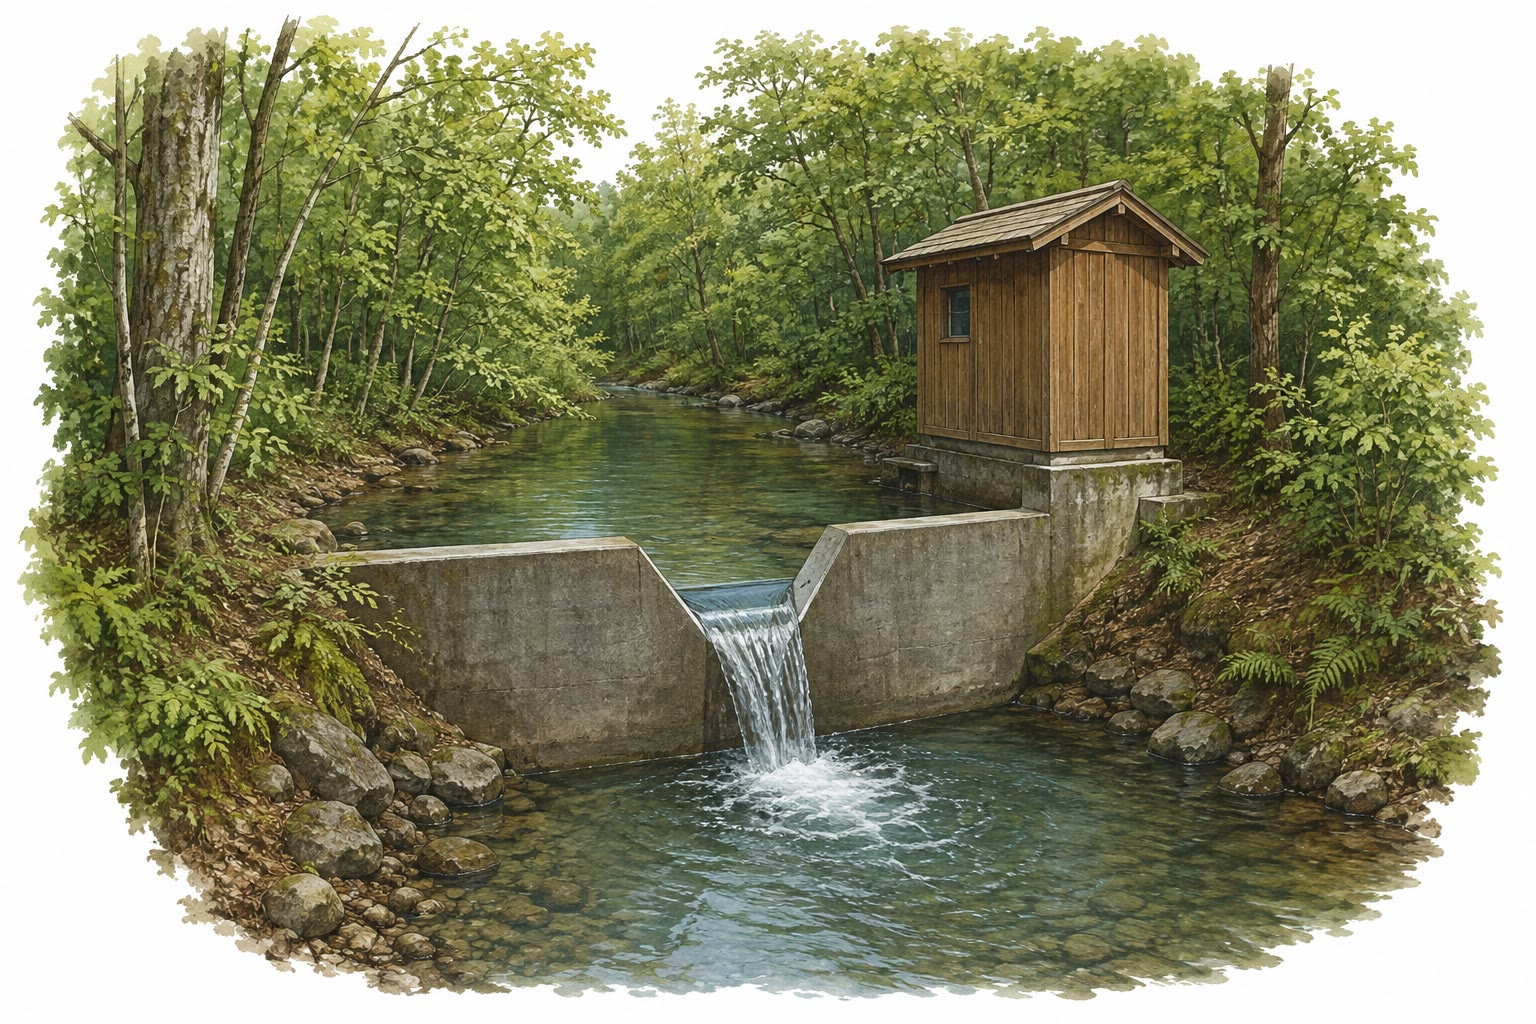
\includegraphics[width=0.56\linewidth]{images/book3/ai/b3-28-stream-weir.jpg}

{\small 量水堰位于森林山谷的出口处，是水体与溶解养分的唯一出口，
在此可测定整个\omterm{def:b1:ecosystem-organization:ecosystem}{生态系统}的
\omterm{def:b1:ecosystem-dynamics:decomposition}{养分收支}。}
\end{omfigure}

\begin{definition}[生态系统工程师]\label{def:b1:ecosystem-dynamics:engineers}
\index{生态系统工程师}
\emph{\omterm{def:b1:ecosystem-organization:ecosystem}{生态系统}工程师}是指为其他物种改变物理\omterm{def:b1:organism-environment:organism}{环境}的物种：
海狸淹没山谷，蚯蚓翻动并
使土壤通气，珊瑚和贻贝构筑礁体，树木遮荫并
保持水分，大象将森林开辟为草原，穴居动物
使沉积物增氧。工程师作用于\omterm{def:b1:ecosystem-organization:ecosystem}{生境}，而非通过营养链发挥作用，
其影响可在其自身消失之后延续（例如海狸草甸、
礁体、泥炭沼泽）。
\end{definition}

\section{岛屿与群落的组装}

\begin{theorem}[岛屿生物地理学的平衡理论]\label{thm:b1:ecosystem-dynamics:island}
\index{岛屿生物地理学}\index{物种–面积关系}
岛上的物种数是动态平衡的结果，
这一平衡发生于来自含 $P$ 个物种的源库的迁入与
岛上的灭绝之间。若新物种的迁入速率随
已存在的物种数 $S$ 线性下降，即 $I = I_0(1 - S/P)$，且灭绝速率
随之线性上升，即 $E = eS$，平衡态为
\[
S^* = \frac{I_0 P}{I_0 + eP} ,
\]
当 $I = E$ 时达到平衡，此时每单位时间有 $eS^*$ 个物种持续更替。
靠近源库的岛屿具有较高的 $I_0$，物种也更多；
大岛的 $e$ 较低（\omterm{def:b1:populations:population}{种群}更大），物种同样更多。
对一组岛屿而言，物种数随面积增长，
按 $S = cA^z$ 变化，在双对数坐标下为斜率为 $z$ 的直线，
其中 $z$ 通常介于 \num{0.2} 与 \num{0.35} 之间。
\end{theorem}
\begin{proof}[部分证明]
$S$ 在迁入超过灭绝时增加，在灭绝超过迁入时减少，
因此 $\dd S/\dd t = I_0(1 - S/P) - eS$ 是一阶线性方程，
其唯一平衡点为 $I_0 -
(I_0/P + e)S = 0$ 的解 $S^*$，且该平衡点是稳定的，因为变化率
在平衡点以下为正，以上为负。平衡时物种仍在
以速率 $eS^*$ 不断迁入与灭绝：物种数恒定，
而物种名录并不恒定。幂律是经验性的，其指数在
\num{0.25} 附近意味着，面积大十倍的岛屿约拥有 \num{1.8}
倍的物种数，而丧失 \qty{90}{\%} 的\omterm{def:b1:ecosystem-organization:ecosystem}{生境}将
最终损失约一半的物种。
\end{proof}
\begin{proof}[证据]
Simberloff 与 Wilson（1969）统计了佛罗里达外海小型红树林小岛上的节肢动物物种，
将这些小岛熏蒸以杀死所有动物，
并间隔一段时间重新统计。一年之内，每个小岛的物种数
都已恢复到接近原有水平——靠近源库和较大的小岛恢复得更多，
远离源库和较小的小岛恢复得较少——但物种名录已不相同，
且名录仍在持续更替：物种数处于平衡，
而物种组成处于更替之中，正如理论所要求的那样。
克拉卡托火山于 1883 年爆发后被灭菌，三年后有 \num{30} 种植物，
五十年后超过 \num{270} 种，接近附近类似岛屿的
\omterm{def:b1:ecosystem-organization:diversity}{物种丰富度}。
\end{proof}

\begin{omfigure}
\begin{tikzpicture}[font=\footnotesize, >=Stealth, line cap=round]
  \draw[->, thick] (0,0) -- (7.0,0) node[below right] {岛上物种数 $S$};
  \draw[->, thick] (0,0) -- (0,4.4) node[above] {速率};
  \node[anchor=north] at (6.0,-0.1) {$P$};
  \draw[very thick, omDef] (0,3.8) -- (6.0,0) node[pos=0.1, above right, omDef!80!black] {迁入，近岛};
  \draw[very thick, omDef, dashed] (0,2.2) -- (6.0,0) node[pos=0.2, below, omDef!80!black] {远岛};
  \draw[very thick, omThm] (0,0) -- (6.0,4.0) node[right, omThm!80!black, align=left] {灭绝，\\ 小岛};
  \draw[very thick, omThm, dashed] (0,0) -- (6.0,2.0) node[right, omThm!80!black, align=left] {灭绝，\\ 大岛};
  \fill (3.0,1.9) circle (2pt); \draw[dashed, gray] (3.0,1.9) -- (3.0,0) node[below, black] {$S^*$};
  \fill (4.6,0.9) circle (2pt); \draw[dashed, gray] (4.6,0.9) -- (4.6,0);
  \fill (1.85,0.63) circle (2pt);
  \node[anchor=north, align=center, gray] at (3.5,-0.55) {平衡点位于两线交点：\\ 近源大岛最高，远岛小岛最低};
\end{tikzpicture}

{\small \omterm{thm:b1:ecosystem-dynamics:island}{岛屿生物地理学}的平衡模型：新物种的迁入
率随已有物种数增加而下降，灭绝率随之上升。
近源抬高迁入线，面积增大则降低灭绝线，
每一对直线确定一个平衡点。}
\end{omfigure}

\begin{omfigure}
\begin{tikzpicture}
\begin{loglogaxis}[
  width=0.74\linewidth, height=5.8cm,
  axis x line=bottom, axis y line=left,
  xmin=0.5, xmax=20000, ymin=8, ymax=200,
  xlabel={岛屿面积（\unit{km^2}）}, ylabel={物种数},
  xlabel style={font=\small}, ylabel style={font=\small},
  tick label style={font=\small},
  log ticks with fixed point,
  legend style={font=\scriptsize, at={(0.03,0.97)}, anchor=north west, draw=none, fill=none},
  legend cell align=left,
]
\addplot[only marks, mark=*, omDef] coordinates {(1,12) (10,21) (100,38) (1000,68) (10000,120)};
\addlegendentry{群岛中的各岛}
\addplot[omThm, thick, domain=0.5:20000, samples=40] {12*x^0.25};
\addlegendentry{$S = 12\,A^{0.25}$}
\end{loglogaxis}
\end{tikzpicture}

{\small 对数坐标上的物种–面积关系为一条直线，
斜率 $z = 0.25$，故面积扩大十倍时，物种数仅增至 \num{1.8}
倍。}
\end{omfigure}

\begin{proposition}[破碎化]\label{prop:b1:ecosystem-dynamics:fragmentation}
\index{栖息地破碎化}
被切割成片段的\omterm{def:b1:ecosystem-organization:niche}{栖息地}如同群岛：每个
片段的物种数向其面积与隔离程度决定的平衡下降，
起初缓慢（\emph{灭绝债务}），体型大、
稀有且特化的物种先消失。片段还会获得边缘效应——更干燥、
风更大、受扰动更多——以内部面积为代价；
面积为 \qty{1}{km^2}、边缘带宽为 \qty{100}{m} 的正方形片段，
其内部仍占面积的 \qty{64}{\%}；而面积为 \qty{0.1}{km^2} 的片段仅
保留 \qty{15}{\%}。片段间的廊道提高迁入速率，
这正是它们恢复物种的速度快于增加面积的原因。
\end{proposition}

\begin{method}[利用物种–面积关系]\label{met:b1:ecosystem-dynamics:sar}
\begin{enumerate}
  \item 对一组以同等努力量取样的岛屿或片段，作 $\log S$ 对 $\log A$ 的图；
        用目测或
        最小二乘法拟合直线。
  \item 读取斜率为 $z$，$c$ 为 $S$ 在 $A = 1$ 时的值。
  \item 将新面积的物种数预测为 $cA^z$；面积由 $A_0$ 减至 $A$ 时，
        保留的物种比例为 $(A/A_0)^z$——取 $z = 0.25$，
        若保留十分之一的\omterm{def:b1:ecosystem-organization:niche}{栖息地}，
        则最终保留 \qty{56}{\%} 的物种。
  \item 注意：只有在灭绝债务偿清后，损失才会显现，
        有时要延迟数十年；拟合本身也不能说明
        哪些物种会消失。
\end{enumerate}
\end{method}

\section{练习}

\begin{exercise}[$\star$]\label{exo:b1:ecosystem-dynamics:1}
区分\omterm{def:b1:ecosystem-dynamics:succession}{初生演替}与\omterm{def:b1:ecosystem-dynamics:succession}{次生演替}，各举一例，
并说明哪种\omterm{def:b1:ecosystem-dynamics:succession}{演替}更快及其原因。
\end{exercise}

\begin{exercise}[$\star$]\label{exo:b1:ecosystem-dynamics:2}
写出物种更替的三种机制，并给出
在新鲜熔岩流上占主导的那一种。
\end{exercise}

\begin{exercise}[$\star$]\label{exo:b1:ecosystem-dynamics:3}
定义\omterm{def:b1:ecosystem-dynamics:disturbance}{抗性}和\omterm{def:b1:ecosystem-dynamics:disturbance}{恢复力}，并对珊瑚礁（再生缓慢、
易白化）和草甸进行分类。
\end{exercise}

\begin{exercise}[$\star$]\label{exo:b1:ecosystem-dynamics:4}
已知 $S = 12 A^{0.25}$，计算面积为
\qty{16}{km^2} 和 \qty{625}{km^2} 的岛屿上的预期物种数。
\end{exercise}

\begin{exercise}[$\star\star$]\label{exo:b1:ecosystem-dynamics:5}
为何冰川湾的云杉在年轻的冰碛土上
只有施用氮肥才能生长，这对桤木说明了什么？
\end{exercise}

\begin{exercise}[$\star\star$]\label{exo:b1:ecosystem-dynamics:6}
一个源库含 200 个物种；空岛每年迁入 $I_0 = 8$ 个
新物种，已有物种每年以 $e = 0.05$ 的比例灭绝。
计算平衡时的物种数，以及平衡时的更替速率。
对距离为两倍的岛屿（$I_0 = 4$）重复上述计算。
\end{exercise}

\begin{exercise}[$\star\star$]\label{exo:b1:ecosystem-dynamics:7}
试从吸收与矿化作用的角度解释，为何被砍伐的
哈伯德溪河谷流失的是硝酸盐而非有机氮，
以及植被重新生长后，流失为何停止。
\end{exercise}

\begin{exercise}[$\star\star$]\label{exo:b1:ecosystem-dynamics:8}
一层叶\omterm{def:b1:ecosystem-dynamics:decomposition}{凋落物}第一年失去 \qty{50}{\%} 的质量。若
\omterm{def:b1:ecosystem-dynamics:decomposition}{分解}为一级反应，求速率常数，以及三年后剩余的比例；
并与针叶树\omterm{def:b1:ecosystem-dynamics:decomposition}{凋落物}作比较，
后者每年失去 \qty{15}{\%}。
\end{exercise}

\begin{exercise}[$\star\star$]\label{exo:b1:ecosystem-dynamics:9}
运用\omterm{prop:b1:ecosystem-dynamics:idh}{中度干扰假说}，预测草原
的多样性随放牧强度由无增至重度的变化，
并解释两端的情形。
\end{exercise}

\begin{exercise}[$\star\star\star$]\label{exo:b1:ecosystem-dynamics:10}
一片面积为 \qty{1000}{km^2} 的森林被破碎为十个
面积为 \qty{10}{km^2} 的片段。取 $z = 0.25$，计算
单个片段中的预期物种数，以及十个片段彼此完全隔离时的总物种数，
与原有森林作比较，并解释为何总和并不是正确答案。
\end{exercise}

\begin{exercise}[$\star\star\star$]\label{exo:b1:ecosystem-dynamics:11}
辛伯洛夫–威尔逊小岛在
一年内恢复了物种数，但物种组成不同。解释
为何这一结果比原有物种名录的完全恢复
更能支持平衡理论。
\end{exercise}

\begin{exercise}[$\star\star\star$]\label{exo:b1:ecosystem-dynamics:12}
“顶极森林是一个封闭系统。”试结合
哈伯德溪的收支数据加以讨论：何物输入，何物输出，何物被循环利用，
以及砍伐实验表明氮的截留来自何处。
\end{exercise}

\section{问题：砍伐的河谷与群岛}

\begin{problem}[{周末问题——砍伐河谷的养分收支，
以及群岛的物种–面积律，
最终落到指数 $z$ 与
小岛的平衡物种数}]
\label{pb:b1:ecosystem-dynamics:1}

\medskip
\noindent\textbf{第一部分——读解\omterm{def:b1:ecosystem-dynamics:succession}{演替}。}
按冰川退缩后的已知年龄排列的一组样地，
数据如下：10 年时，有苔藓和一层\omterm{def:b1:plant-water-minerals:nodules}{固氮}生物，土壤氮
含量为 \qty{10}{kg/ha}；40 年时，为桤木灌丛，\qty{150}{kg/ha}；
80 年时，为云杉林，\qty{300}{kg/ha}；200 年时，
为云杉–铁杉林，\qty{320}{kg/ha}。
\begin{enumerate}
  \item 计算每个时段内氮积累的平均速率，
        并指出何时最快。
  \item 氮的曲线指向哪一种替代机制，
        对应哪一次更替？
  \item 为何 80 年后氮的积累几乎停止，
        尽管森林仍然存活？
  \item 桤木每年固定 \qty{50}{kg/ha} 的氮。其中
        有多大比例在第 40 至 80 年间保留在土壤中，
        其余去向何处？
  \item 设计一个实验，以区分桤木向云杉更替过程中的促进
        作用与耐受作用。
  \item 时序样地为何只能替代、而不等同于
        连续两个世纪观察同一地点？
\end{enumerate}

\medskip
\noindent\textbf{第二部分——砍伐后的河谷。}
两个相邻河谷各为 \qty{15}{ha}，每年接收 \qty{1300}{mm}
的降雨，雨水中溶有 \qty{6.5}{kg/ha} 的氮。
林覆的对照河谷每年输出 \qty{820}{mm} 的溪水，
其中含 \qty{2}{kg/ha} 的硝酸盐氮、\qty{9}{kg/ha} 的钙，
和 \qty{2}{kg/ha} 的钾。砍伐河谷在砍伐后第二年，
输出 \qty{1150}{mm} 的溪水，其中含 \qty{120}{kg/ha} 的
硝酸盐氮、\qty{90}{kg/ha} 的钙和 \qty{36}{kg/ha} 的
钾。其土壤与\omterm{def:b1:ecosystem-dynamics:decomposition}{凋落物}含氮 \qty{3500}{kg/ha}，
被砍伐的生物量另含 \qty{350}{kg/ha} 的氮。
\begin{enumerate}[resume]
  \item 产水量上升了多少？原因何在？
  \item 计算每条溪流中硝酸盐氮的平均浓度，
        单位为毫克每升（\qty{1}{mm} 的水分布于 \qty{1}{ha} 上，
        即为 \qty{10}{m^3}）。
  \item 计算每个河谷的氮收支（输入减输出），
        哪一个河谷在积累氮？积累速率为多少？
  \item 砍伐河谷的土壤氮中，有多大比例在
        那一年内流失？若按此速率，该氮库能维持多久？
  \item 钙和钾的输出分别上升了多少倍？
        为何钾的上升幅度大于钙？（考虑两者在土壤中
        各自的保持位置。）
  \item 输出的硝酸盐从何而来，既然没有植被
        生长以释放氮？请说出两个微生物
        步骤。
  \item 允许植被再生后，输出在第 4 年降至 \qty{20}{kg/ha}，
        第 6 年降至 \qty{5}{kg/ha}。降雨输入需多久
        才会再次超过输出？是什么恢复了
        氮的截留？
\end{enumerate}

\medskip
\noindent\textbf{第三部分——群岛。}
五个小岛的面积分别为 \qtylist{1;10;100;1000;10000}{km^2}，各载陆生鸟类 \num{12}、\num{21}、\num{38}、\num{68} 和
\num{120} 种。大陆物种库含 \num{300}
个物种。
\begin{enumerate}[resume]
  \item 计算各面积与各物种数的 $\log_{10}$，并
        作图。
  \item 由两个端点求出 $z$，由最小的小岛求出 $c$；
        检验中间各岛是否符合。
  \item 预测面积为 \qty{250}{km^2} 的小岛的物种数。
  \item 面积为 \qty{100}{km^2} 的小岛在空岛时每年迎来 $I_0 = 6$ 个新物种，
        并每年以比例 $e$ 失去其物种。
        取 $S^* = 38$，求 $e$ 以及平衡时的更替速率。
  \item 距离为两倍的同面积小岛，其 $I_0 = 3$。
        取相同的 $e$，求其平衡物种数。
  \item 一座桥梁将面积为 \qty{100}{km^2} 的小岛与大陆相连，
        $I_0$ 升至 \num{30}。求新的平衡物种数，并
        解释为何它仍远低于 \num{300}。
  \item 若 $z$ 为 \num{0.35} 而非 \num{0.25}，小岛
        相对大岛会有更多还是更少的物种？说明
        高 $z$ 在生物学上意味着什么。
\end{enumerate}

\medskip
\noindent\textbf{第四部分——破碎化与恢复。}
\begin{enumerate}[resume]
  \item 计划在一片本将被砍伐的森林中划出面积为 \qty{1000}{km^2} 的保护区。
        该森林面积为 \qty{100000}{km^2}，取 $z =
        0.25$，该保护区最终能容纳
        该森林物种的多大比例？
  \item 若十个面积为 \qty{100}{km^2} 的保护区彼此隔离，
        所容纳的物种数会更多还是更少？若以廊道相连，又如何？
  \item 保护区的边缘带宽为 \qty{300}{m}。计算
        面积为 \qty{1000}{km^2} 的方形保护区的内部比例，以及
        面积为 \qty{100}{km^2} 的方形保护区的内部比例。
  \item 画出新隔离片段的物种数随时间变化的示意图，
        并解释“灭绝债务”一词。
  \item 陈述结果：群岛的指数 $z$，以及
        面积为 \qty{100}{km^2} 的小岛在建桥前后的
        平衡物种数。
\end{enumerate}
\end{problem}
